\documentclass[letterpaper,twocolumn,superscriptaddress,showkeys]{revtex4}
\usepackage[utf8]{inputenc}
\usepackage{color,dcolumn,graphicx,hyperref}
\hypersetup
{
    colorlinks = true, linkcolor = blue, citecolor = blue, urlcolor = blue,
}

\begin{document}

\title{Open Preprints in Ecology \& Evolution}

\author{Philippe Desjardins-Proulx}
\email[E-mail: ]{philippe.d.proulx@gmail.com}
\affiliation{Theoretical Ecosystem Ecology laboratory, Universit\'e du Qu\'ebec \`a Rimouski, Canada.}
\affiliation{Quebec Center for Biodiversity Science, McGill University, Canada.}
\affiliation{D\'epartement des sciences biologiques, Universit\'e du Qu\'ebec \`a Montr\'eal, Canada.}

\author{Ethan P. White}
\affiliation{Departement of Bology, Utah State University, United-States of America.}

\author{Timoth\'ee Poisot}
\affiliation{Theoretical Ecosystem Ecology laboratory, Universit\'e du Qu\'ebec \`a Rimouski, Canada.}
\affiliation{Quebec Center for Biodiversity Science, McGill University, Canada.}
\affiliation{International Network for Next-Generation Ecology.}

\author{Dominique Gravel}
\affiliation{Theoretical Ecosystem Ecology laboratory, Universit\'e du Qu\'ebec \`a Rimouski, Canada.}
\affiliation{Quebec Center for Biodiversity Science, McGill University, Canada.}

\keywords{Publishing; arXiv; Green Open Access.}

\begin{abstract}

...
 
\end{abstract}

\maketitle

\section{The case for open preprints}

Preprints servers such as arXiv are common in mathematics and physics, but still
a minority of papers in ecology and evolution use them. Preprints servers allow
author to make their manuscripts publicly available before submitting them to
journals for peer-review. ... The idea became popular with arXiv, and many
physicists start their day with a look at the new papers in arXiv \cite{gin11}

We will highlight advantages for both scientists and publishers.

The first and most often discussed advantage is speed \ref{fig:map}.

%% Allows papers to be cited earlier (greater immediacy)

%% @Tim: how can it improve the review process?

\begin{figure}[ht!] \centering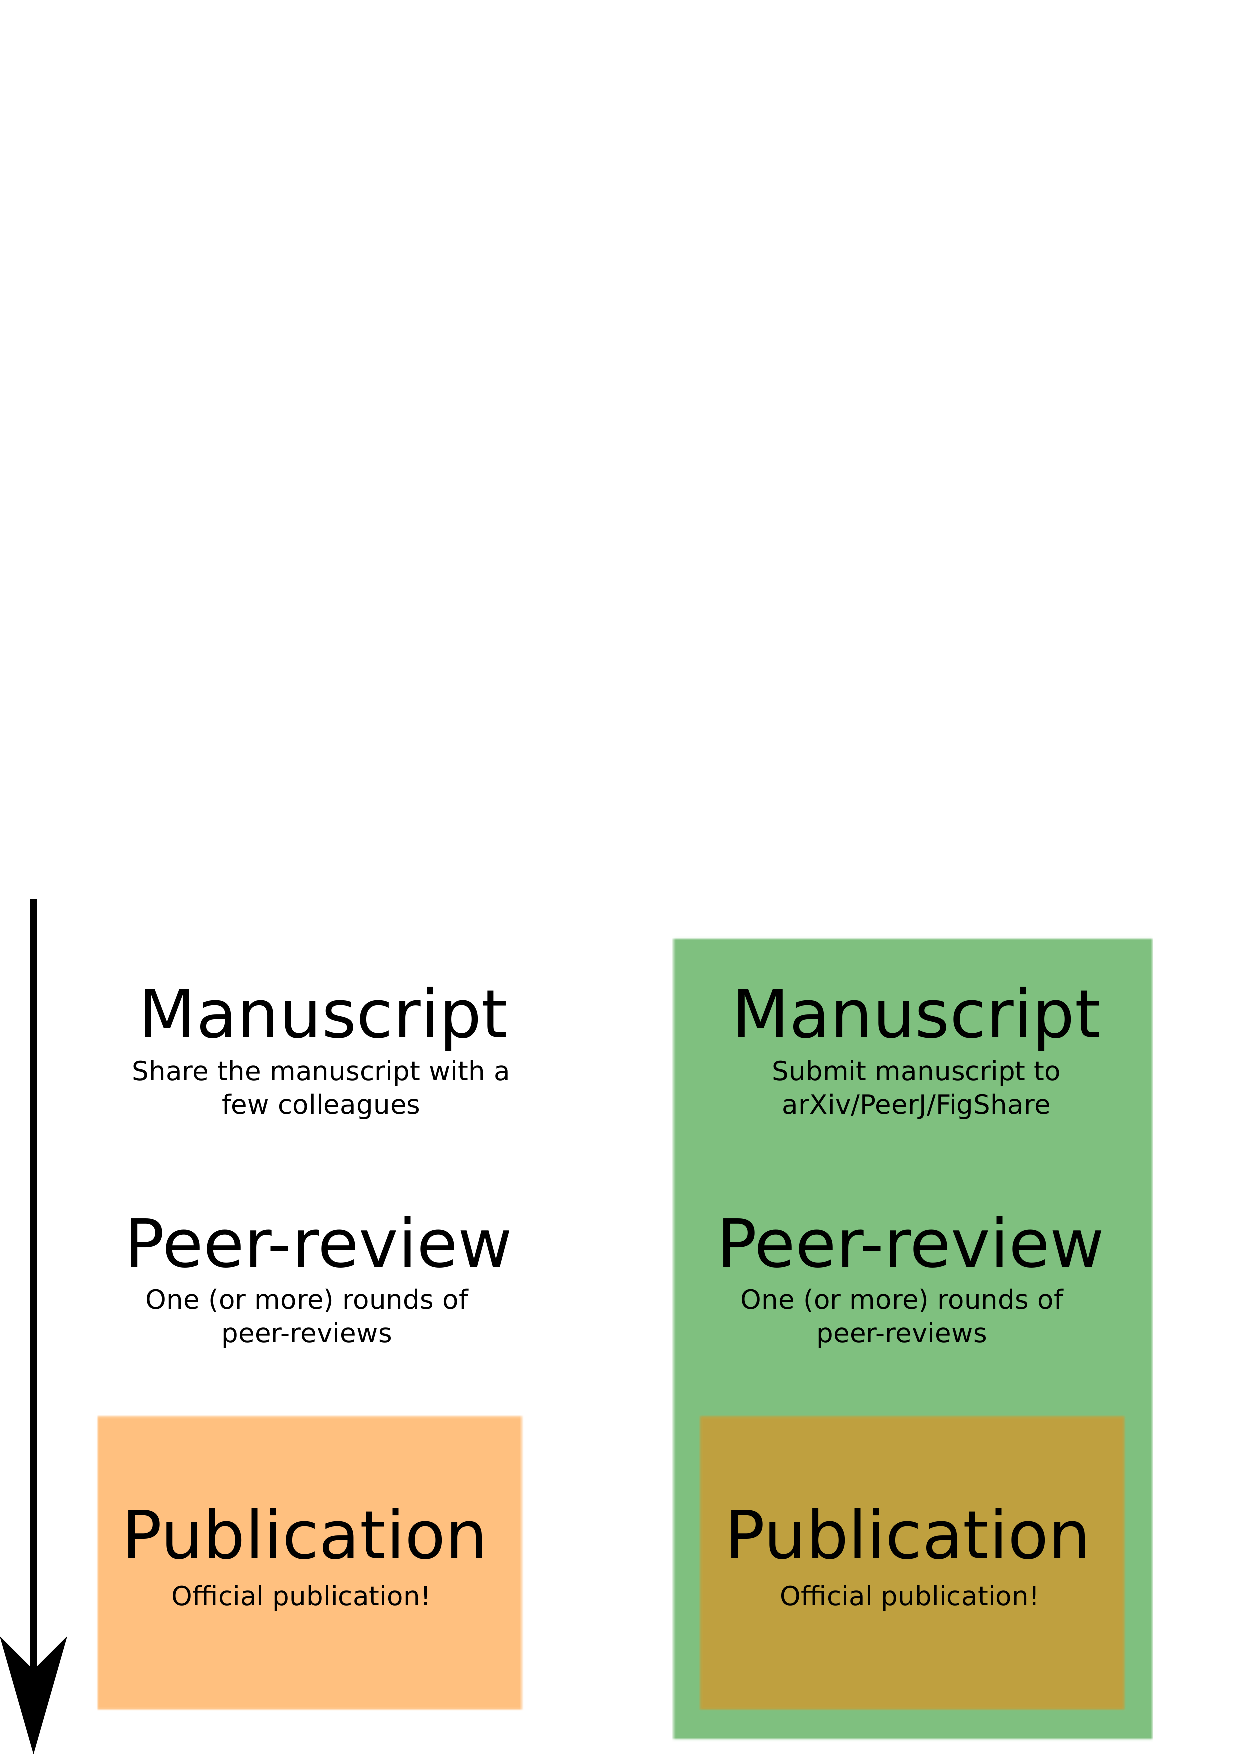
\includegraphics[width=0.50\textwidth]{map.pdf}
\caption { It can take several months, and even a few years, before a submitted
paper is officially published. During this time, few people are aware of the
research that has been done. With public preprint servers, the science is
immediately available and can be openly discussed, analysed, and integrated into
current research. It benefits both science and publishers. Both want the papers
to be well-known and cited, and public preprints make it possible to integrate
research even before publication, improving immediacy.  } \label{fig:map}
\end{figure}

Preprint servers also establish priority in a fair way. Some manuscript will
spend much more time in the review process. Public preprints server offer a much
fairer way to establish intellectual priority By making the manuscript available
when it is ready. Surprisingly, there is perception in biology that public
preprints make it easier to steal ideas, as if scientific ideas only took form
in published material. Mathematicians and physicists have embraced arXiv in part
to establish priority in a fair way\cite{cal12}.

Some of the responses to public preprints are surprisingly since they are,
essentially, the same as exchanging preprints among colleagues. Prepublication
reviews by a small network of colleagues is an important part of the scientific
process. Preprints servers simply offer a way to extend this network of
colleagues to the entire scientific community. It ensures that science is not
constrained by small networks of scientists exchanging ideas. Ginsparg made
arXiv.org in part for democratic reasons: he wanted everyone from graduate
students in small universities to Princeton professors to have access to the
most recent scientific ideas. Ginsparg revolutionary idea was simply to use the
power of the internet for preprints, not just for the end product, so the
process can be open from A to Z, instead of being just open at the end of the
process.

\section{Preprints, Ecology \& Evolution}

While the practice is still rare, preprints are becoming more common in
biological sciences, which is experiencing faster growth in arXiv submissions
than any other fields \cite{cal12}. Also, most scientific journals are
preprint-friendly: Nature, PLOS, BMC, PNAS, Science (mostly)
\ref{table:policies}, and all the journals from Elsevier and Springer. Very
recently, the Ecological Society of America recently changed its policy to allow
public preprints (REF). In our field, few scientific publications will not
consider a manuscript submitted to arXiv. Still, many ecology \& evolution journals
adopt a ``by default'' hostile attitude towards preprints, mostly due to the
lack of clear policy of the publishers. As an example, Wiley-Blackwell, which
publishes some of the leading journal in the field, has no official policy on
the subject \ref{table:policies}.

\begin{table*}
    \centering
    \begin{tabular}{|ll|}
    \hline
    Publisher                                   & Policy \\
    \hline
    Springer                            	& Accept \\
    BMC                                 	& Accept \\
    Elsevier                            	& Accept \\
    Nature Publishing Group             	& Accept \\
    Public Library of Science           	& Accept \\
    Royal Society                       	& Accept \\
    National Academy of Science (USA)           & Accept \\
    Science                             	& Accept/Ambiguous \\
    Wiley-Blackwell                       	& No general policy \\
    Ecological Society of America       	& Refuse \\
    British Ecological Society                  & ? \\
    \hline
    \end{tabular}
    \caption{Policies for important publishers in ecology and evolution.}
    \label{table:policies}
\end{table*}

\section{Current offer}

We briefly discuss the main options to submit preprints to open servers:
arXiv.org, Figshare, and the upcoming PeerJ and F1000Research.

\subsection{arXiv}

arXiv (\href{http://arxiv.org/}{http://arxiv.org/}).
arXiv is funded by a network of universities.

...

% @Joel

\subsection{Figshare}

% @PhDP

Figshare (\href{http://figshare.com/}{http://figshare.com/})

All figshare content (article, figures, datasets) have a unique digital object
identifier (DOI) like any journal article.

\subsection{PeerJ}

% @Ethan

\subsection{F1000Research}

% Written from memory: to verify!

F1000Research is not a public preprint server like the previous three servers.
Whereas arXiv, Figshare, and PeerJ offer an option to submit a manuscript
without having it reviewed, papers submitted to F1000Research will eventually be
reviewed. Thus, F1000Research offers a hybrid model with publicly available
manuscripts at time of submission and standard peer-reviews. Manuscripts are
considered ``accepted'' and will only be indexed after two positive referee
response.

\section{Conclusion}

% A short paragraph to conclude.

Responding to the rumour that they refused manuscripts submitted to arXiv,
Nature responded that ``Nature never wishes to stand in the way of communication
between researchers. We seek rather to add value for authors and the community
at large in our peer review, selection and editing'' \cite{nat05}.

\newpage
\bibliography{refs}
\bibliographystyle{plain}

\end{document}

